\documentclass{beamer}

\usepackage[french]{babel}
\usepackage[T1]{fontenc}
\usepackage[utf8]{inputenc}
\usepackage{graphicx}
\usepackage{hyperref}
\hypersetup{colorlinks,urlcolor=blue}

\usetheme{Singapore}


\title{Caractériser les adhérents de la Médiathèque de Roubaix selon leur lieu d'habitation}
\subtitle{Approches quantitatives et modélisation mathématique en SHS}
\author{François Pichenot}
\institute{Université Paris Sciences et Lettres - École nationale des chartes\\Master Humanités numériques et computationnelles}
\date{16 janvier 2020}

\begin{document}

% page de titre
\begin{frame}
	\titlepage
\end{frame}

% pages
\begin{frame}{Le problème}
	\begin{itemize}
    	\item des données en lien avec le projet de recherche encore mal cernées,
    	\item on abordera donc un problème en lien avec le contexte professionnel des bibliothèques :
    	\begin{itemize}
    		\item caractériser les pratiques des adhérents selon leur provenance géographique (quartier)
    	\end{itemize}
	\end{itemize}
\end{frame}

\begin{frame}{Le problème (contextualisation)}
	\begin{itemize}
    	\item Roubaix : une ville contrastée
    	\begin{itemize}
    		\item la majeure partie des habitants connaissent de graves difficultés économiques et sociales,
    		\item mais une moindre partie jouit de conditions matérielles plus favorables
    	\end{itemize}
    	\item des inégalités qui transparaissent dans la géographie :\\voir la carte suivante, on essaie de représenter les différences du revenu fiscal médian par unité de consommation (source : INSEE 2011) en l’exprimant au moyen d’un indice, l’indice 1 équivalent à la médiane).
	\end{itemize}
\end{frame}

\begin{frame}{Le problème (contextualisation)}
	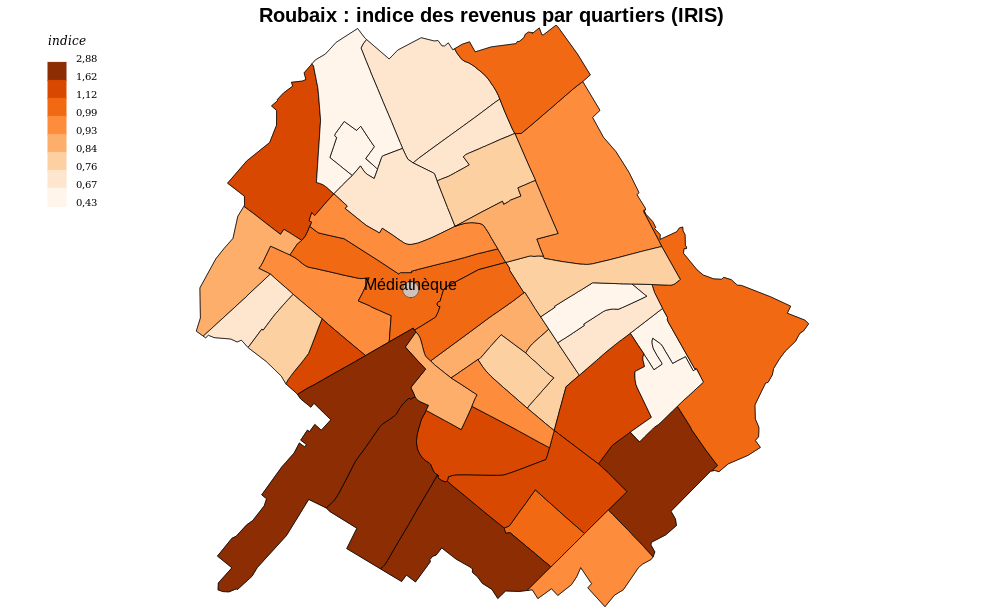
\includegraphics[scale=0.35]{/home/fpichenot/enc/cours/S3_Modelisation_mathematique/RBX/presentation/data/iris_carte_revenus.png}
\end{frame}

\begin{frame}{Le problème (contextualisation)}
	\begin{itemize}
    	\item Une bibliothèque municipale (médiathèque) située en centre ville (un seul site) :
    	\begin{itemize}
    		\item qui a des difficultés à toucher les habitants des quartiers éloignés du centre ville,
    		\item qui a besoin de mieux connaître les pratiques (donc les attentes) des habitants qui la fréquentent en fonction du quartier d’origine.
    	\end{itemize}
    	\item Pour appréhender les pratiques, on dispose de données d’usage, produites par le système informatique de l’établissement, qui vont permettre de connaître :
    	\begin{itemize}
    		\item le nombre de venues sur une période donnée au sein d l’établissement,
    		\item le type d’activité réalisé
    	\end{itemize}
    	\item Attention : évidemment de nombreux angles morts.
	\end{itemize}
\end{frame}

\begin{frame}{Attentes}
	Être en mesure de faire parler de manière pertinente des données :
	\begin{itemize}
		\item qui décrivent un échantillon large (plus milliers d’individus)
		\item qui comportent un nombre important de variables
	\end{itemize}
\end{frame}

\begin{frame}{Les données}
	On part d'un \href{https://opendata.roubaix.fr/explore/dataset/caracteristiques_adherents_2018}{jeu de données} mis en ligne sur la plateforme open data de la Ville de Roubaix :
	\begin{itemize}
		\item il a vocation à décrire les caractéristiques des adhérents de la Médiathèque de Roubaix.
		\item il s'agit de données structurées (élaborées de bases de données relevant d'un système informatique métier) et disponibles sous format tabulé.
	\end{itemize}
	Une exploration détaillée de ces données est proposée \href{https://opendata.roubaix.fr/explore/dataset/caracteristiques_adherents_2018}{ici}.
\end{frame}

\begin{frame}{Que cherche-t-on ?}
	\begin{itemize}
		\item On a montré que le ratio nombre d'inscrits à la Médiathèque / nombre d'habitants pour chaque quartier était très inégal.
		\item On cherche désormais à savoir si, en termes de pratiques, on peut caractériser les différents quartiers.
	\end{itemize}
\end{frame}

\begin{frame}{Approches}
	\begin{itemize}
		\item Approches retenues
		\item Pour aller plus loinss
		\item Approches non pertinentes
	\end{itemize}
\end{frame}

\end{document}